\section{هدف تمرین}
در این تمرین، با تست کردن کد مالتی‌پلکسر 2 به 1 که در کلاس نوشته شد، به بررسی یکی از قواعد کد نویسی قابل سنتز در توصیف رفتاری می‌پردازیم. این قاعده می‌گوید: «هنگام توصیف رفتاری یک مدار ترکیبی بعد از \lr{@} (تنها یک \lr{@} داریم و آن هم پس از \lr{always} هست)، باید \textbf{تمام} ورودی‌های مدار ترکیبی را در \lr{sensitivity list} قرار دهیم.»

\section{کدهای Verilog}

\subsection{ماژول مالتی‌پلکسر (\code{MUX\_2\_1.v})}
در کد این مالتی‌پلکسر (که توصیف رفتاری است) عمداً ورودی \code{sel} (پایه‌ی انتخاب) از \lr{sensitivity list} حذف شده. بنابراین مدار فقط به تغییرات دو ورودی \code{I0} و \code{I1} واکنش نشان می‌دهد و با صرفا تغییر دادن \code{sel}، خروجی مدار تغییر نمی‌کند. کد این ماژول به این صورت می‌باشد:

\begin{latin}
    \begin{lstlisting}[language=Verilog]
module MUX_2_1 (I0, I1, sel, O);

    input [7:0] I0, I1;
    input sel;
    output [7:0] O;
    reg [7:0] O;

    always @(I0, I1)
        if (sel == 1)
            O = I1;
        else
            O = I0;

endmodule
\end{lstlisting}
\end{latin}

بر اساس تعریف، «اگر یک مدار به ازای ورودی‌های کاملاً یکسان در زمان‌های گوناگون خروجی‌های متفاوت داشته باشد، می‌گوییم حافظه دارد.» در این مثال هم چون ورودی \code{sel} از \lr{sensitivity list} حذف شده، به صورت ناخواسته مدار حافظه‌دار شده که می‌توانیم با یک تست‌بنچ این موضوع را نشان دهیم.

\subsection{تست‌بنچ (\code{testbench.v})}
می‌خواهیم در این تست‌بنچ حالتی ایجاد کنیم که به ازای ورودی‌های کاملاً یکسان در زمان‌های متفاوت، ماژول مالتی‌پلکسر دو خروجی متفاوت بدهد. (و نتیجه بگیریم که این ماژول حافظه دارد.) برای این کار می‌توانیم از این استراتژی استفاده کنیم: ابتدا مقادیر اولیه را به \lr{MUX} می‌دهیم ($\text{\code{sel}}=1$)، سپس \code{sel} را تغییر می‌دهیم تا خروجی‌های بعدی از \code{I0} بیایند. برای اینکه مقدار خروجی تغییر کند، باید \code{I0} تغییر کند؛ پس \code{I0} را به یک مقدار ثانویه تغییر داده و سپس به حالت اولیه برمی‌گردانیم تا خروجی آپدیت شود. در نهایت هم $\text{\code{sel}}=1$ می‌کنیم تا ورودی‌ها کاملاً مشابه حالت اولیه شوند.

\begin{latin}
    \begin{lstlisting}[language=Verilog]
`timescale 1ns / 1ns

module testbench;
    reg [7:0] I0;
    reg [7:0] I1;
    reg sel;
    wire [7:0] O;

    MUX_2_1 mux (I0, I1, sel, O);

    initial begin
        $dumpfile("waves.vcd");
        $dumpvars(0, testbench);

        $display("Time\t I0\t I1\t sel\t O");
        $display("-----------------------------------------");
    end

    always @(I0, I1, sel, O) begin
        #0.1; 
        $display("%4dt\t %h\t %h\t  %b\t %h", $time, I0, I1, sel, O);
    end

    initial begin
        I0 = 8'hAA; I1 = 8'hBB; sel = 1;
        #20;

        sel = 0;
        #20;

        I0 = 8'h00;
        #20;
        
        I0 = 8'hAA;
        #20;

        sel = 1;
        #20;

        $finish;
    end
endmodule
\end{lstlisting}
\end{latin}

\subsection{اصلاح مالتی‌پلکسر (\code{MUX\_2\_1\_FIXED.v})}
برای اصلاح ماژول مالتی‌پلکسر، کافی است ورودی \code{sel} را به \lr{sensitivity list} اضافه کنیم. بنابراین کد اصلاح شده به این صورت خواهد بود:

\begin{latin}
    \begin{lstlisting}[language=Verilog]
module MUX_2_1 (I0, I1, sel, O);

    input [7:0] I0, I1;
    input sel;
    output [7:0] O;
    reg [7:0] O;

    always @(I0, I1)   // CHANGED
        if (sel == 1)
            O = I1;
        else
            O = I0;

endmodule
\end{lstlisting}
\end{latin}

\section{اجرای کد}
کدهای نوشته شده را کامپایل و اجرا می‌کنیم. خروجی تست‌بنچ به این صورت می‌باشد:

\begin{figure}[H]
    \centering
    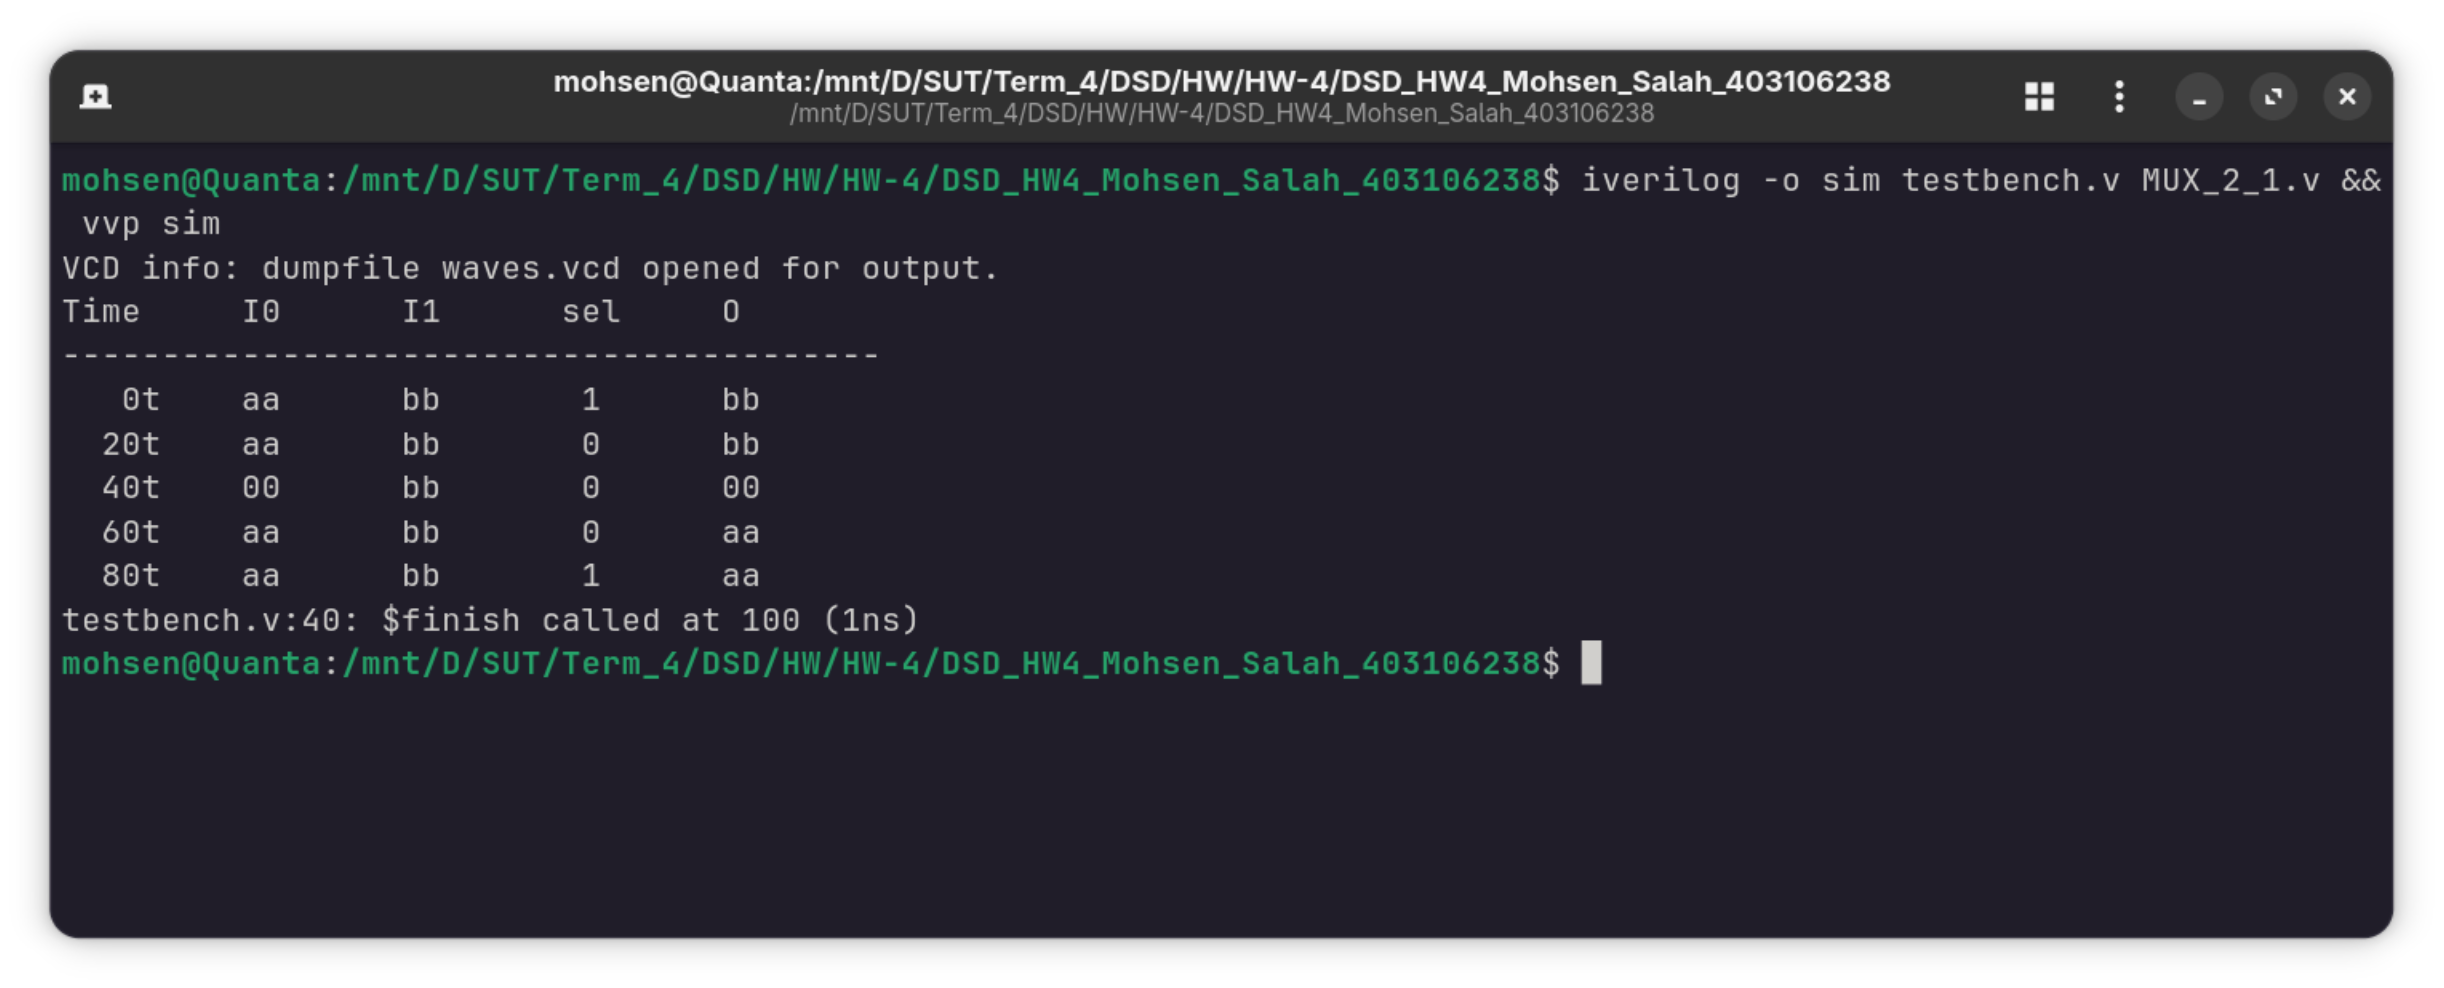
\includegraphics[width=1.0\textwidth]{assets/terminal.png}
    \caption{خروجی تست‌بنچ نوشته شده برای کد اصلی}
\end{figure}

همان طور که مشاهده می‌شود، در زمان‌های 20 و 80، ورودی مالتی‌پلکسر کاملاً یکسان است ($\text{\code{I0 = 0xAA}}$, $\text{\code{I1 = 0xBB}}$, $\text{\code{sel = 1}}$) ولی در زمان 20، \code{O = 0xBB} و در زمان 80، \code{O = 0xAA}. پس خروجی مدار با ورودی‌های کاملاً یکسان در دو زمان مختلف متفاوت است و نتیجه می‌گیریم که مدار حافظه دارد.

\pagebreak

خروجی تست‌بنچ برای نسخه‌ی اصلاح شده نیز به این صورت می‌باشد:

\begin{figure}[H]
    \centering
    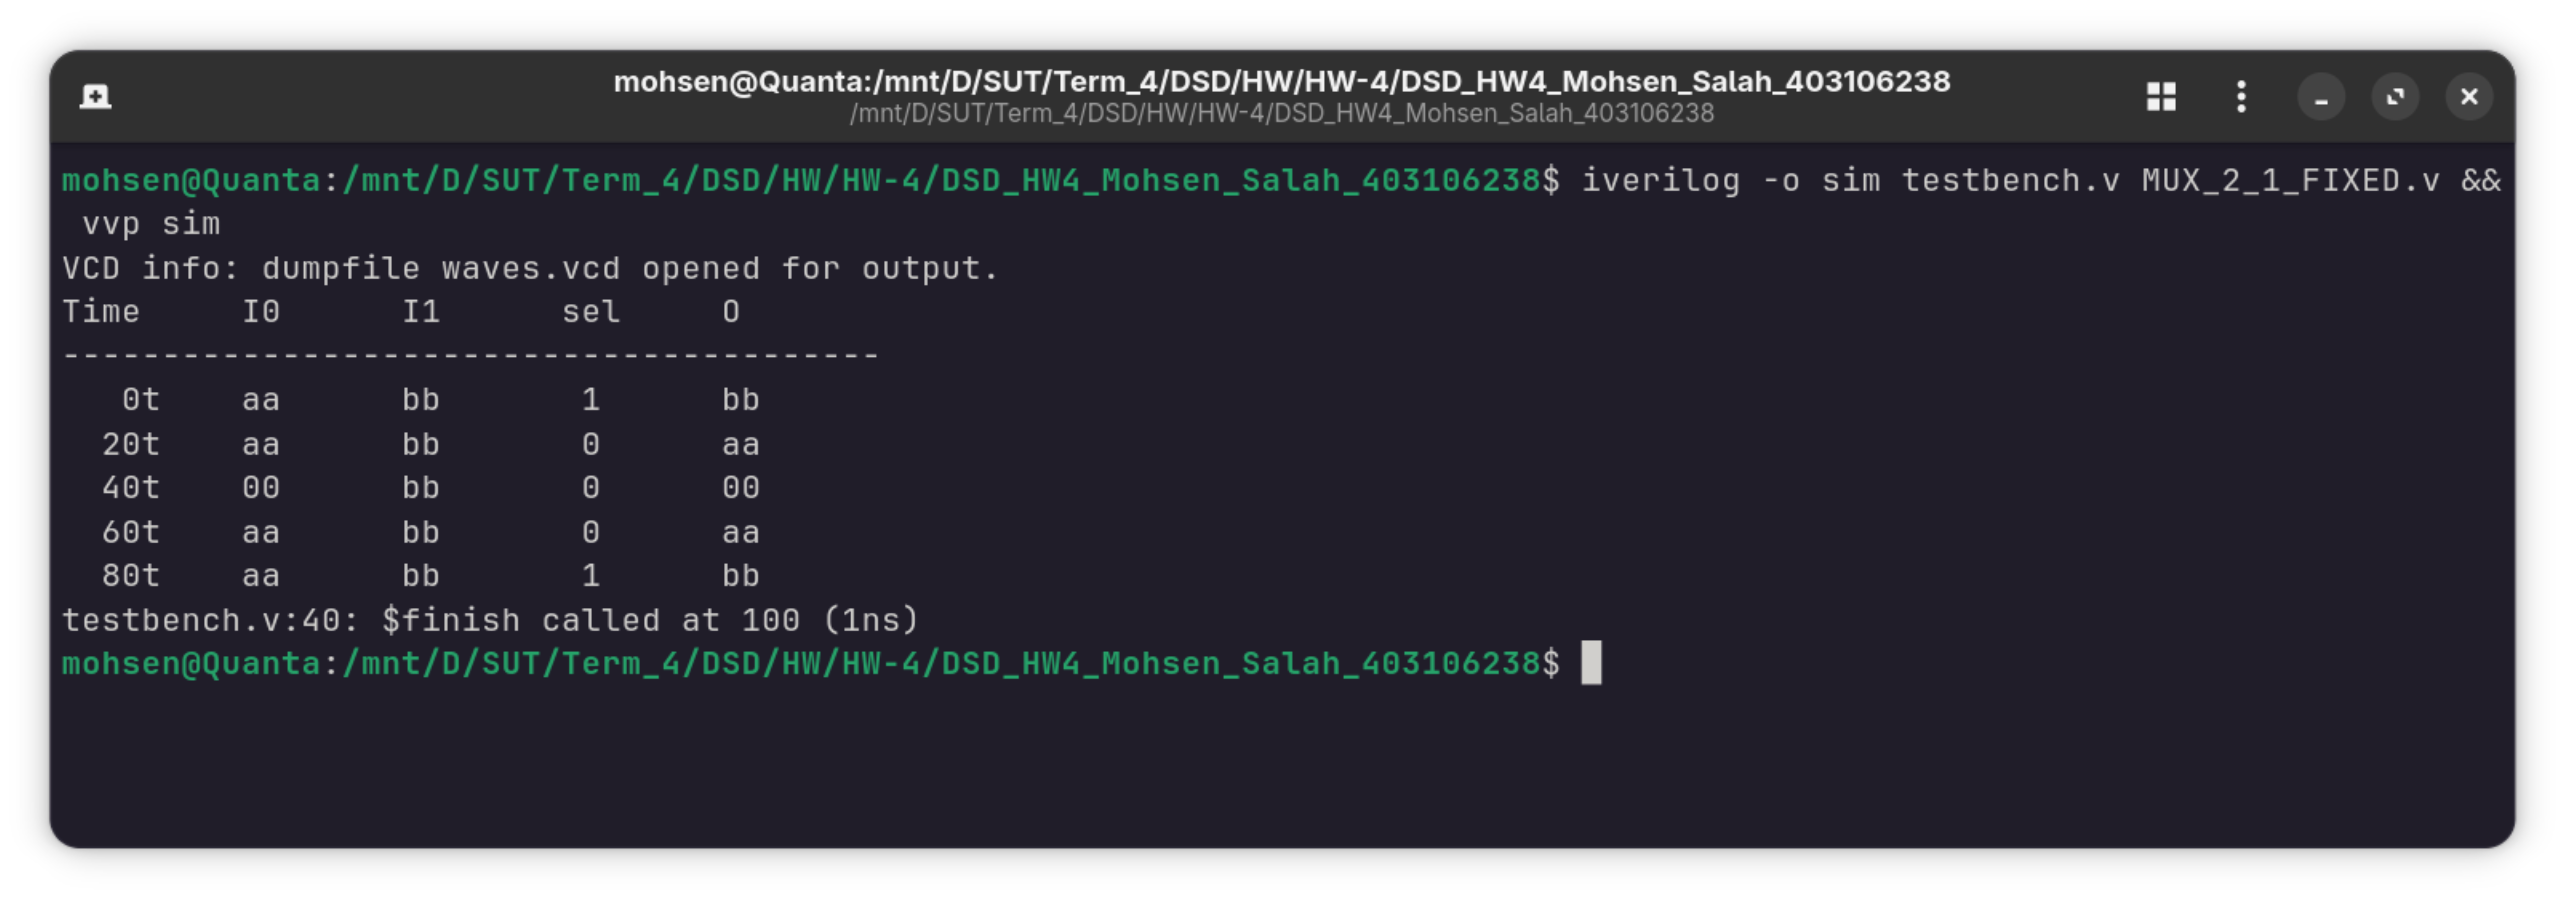
\includegraphics[width=1.0\textwidth]{assets/terminal_changed.png}
    \caption{خروجی تست‌بنچ نوشته شده برای کد اصلاح شده}
\end{figure}

که می‌بینیم در این نسخه کد به درستی عمل کرده و خروجی همواره به صورت ترکیبی از روی ورودی‌ها حاصل شده و مدار حافظه ندارد.

می‌توانیم سیگنال‌های ورودی و خروجی این شبیه‌سازی را در نرم‌افزار \lr{GTKWave} نیز بررسی کنیم:

\begin{figure}[H]
    \centering
    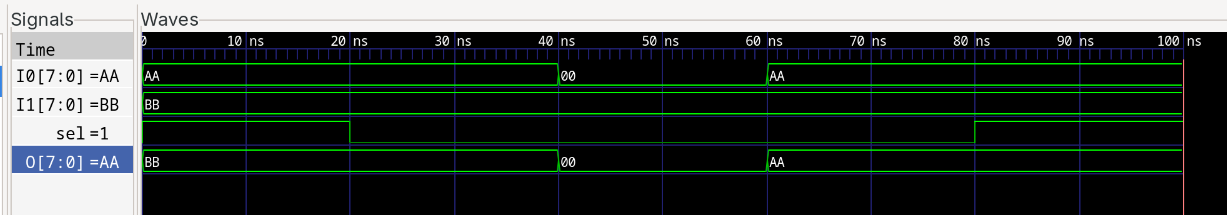
\includegraphics[width=1.0\textwidth]{assets/gtkwave.png}
    \caption{شکل موج سیگنال‌ها در محیط GTKWave برای کد اصلی}
\end{figure}

همان طور که مشاهده می‌شود، خروجی مالتی‌پلکسر به تغییر \code{sel} واکنشی نمی‌دهد. این موضوع باعث شده که عملکرد آن اشتباه باشد و عملاً حافظه داشته باشد، در صورتی که یک مدار ترکیبی است.

شکل موج‌ها برای نسخه‌ی اصلاح شده نیز به این صورت می‌باشد:

\begin{figure}[H]
    \centering
    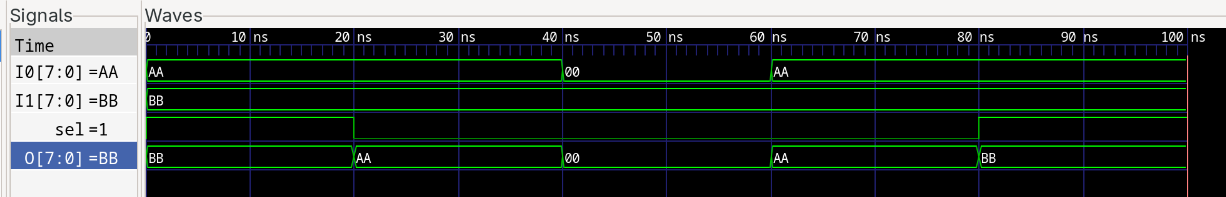
\includegraphics[width=1.0\textwidth]{assets/gtkwave_changed.png}
    \caption{شکل موج سیگنال‌ها در محیط GTKWave برای کد اصلاح شده}
\end{figure}

که روشن است در این نسخه، با عوض شدن مقدار \code{sel}، خروجی نیز تغییر می‌کند و عملکرد مدار صحیح است.